% !TEX root = main.tex

\section{Motivation}

The widespread adoption of the web has emphasized the importance of ensuring that online content is accessible to everyone, including individuals with various disabilities\cite{abu2023web}. Despite this, less than 4\% of the top one million websites are fully accessible. Over 96\% contain detectable \ac{WCAG} failures, with an average of 51 errors per page \cite{webaimmillion2025}. Common issues include missing alt text (present on 56\% of home pages), low contrast, and poor form labeling \cite{audioeye2024}.

On the other hand, rigorous testing is integral to ensuring reliability of web applications. For example, usability testing that involves having real users interacting with a live web application, allows for the identification of issues in action, enables for iterative feedback and a more realistic assessment of how they might experience the interface. Effective testing improves satisfaction, avoids rework, and ensures genuine inclusive design \cite{accessdesign2025}.

% ya se habla de esto bastante
% Although \ac{WCAG} articulate extensive criteria for inclusive design \cite{w3c_WCAG22}, existing tools focus more on compliance than on realistic user behavior. Developers and UX practitioners often lack practical mechanisms to validate these guidelines in realistic usage scenarios. For instance, some of the significant challenges found in testing are little room for iteration, lack of extensive and appropiate user feedback, and limitations to empathy-based research methods\cite{lu2025uxagent}. 

Recent research highlights that most applications of \ac{AI} in web \ac{a11y} focus on generating alternative text for images, automating compliance checks, suggesting corrections, and creating alternative interfaces to improve access\cite{vera2025towards}. However, these approaches remain largely centered on white-box analysis and do not fully address the challenges of evaluating \ac{a11y} from the perspective of real user interaction. 

While recent advances have demonstrated the potential of autonomous agents for usability testing\cite{lu2025uxagent}, mobile \ac{a11y} feature testing\cite{taeb2024axnav} and a11y testing\cite{zhong2025screenaudit}, to our knowledge, these agents have not yet been applied to web \ac{a11y} evaluation in a multi-modal decision-based way. Bridging this gap offers the opportunity to deliver scalable, repeatable, and realistic assessments of how users with disabilities interact with web interfaces, potentially enhancing the detection and remediation of \ac{a11y} issues and making the evaluation process more efficient and comprehensive.

\section{Automated Testing}

Dynamic testing can help developers and stakeholders verify and validate that running software is working as expected\cite{vasquez2018continuous}. In this case, automated testing is the enabler for faster, more reliable and overall optimized testing. Automated testing leveraged by machine learning and \ac{AI} are increasingly becoming more popular and sophisticated, therefore using them in this scenario is a big step forward for ensuring \ac{a11y}.

Intelligent agents can interact with web content without access to the underlying code, relying instead on the same content the final user is interacting with\cite{lanham2025ai, wang2024survey, lu2025uxagent}. They can also be adapted based on feedback, and can process rich multimodal inputs, such as screenshots and screen reader text, enabling them to reason about both the visual layout and the spoken feedback of the user interface simultaneously. They are also able to use different interaction techniques, like keyboard only, mouse only, etc. 

Finally, LLM agents excel at open-ended reasoning and can provide qualitative insights, alongside quantitative logs. However, they require careful prompting and can be slower or less predictable.
\vspace{-8pt}

\section{Objectives}

First, we aim to explore the use of perceptual filters and multimodal inputs, such as applying blur to simulate different impairments; while also using screen reader outputs, to approximate the experience of real world users. 

Additionally, we will analyze whether certain \ac{UI} elements become inaccessible or difficult to perceive under these simulated conditions, and investigate if common layout structures or design patterns can fail in these situations. Through this approach, we seek to identify not only the direct effects of visual filters on usability, but also the broader structural and behavioral implications for accessible web design.

\section{System design}
\subsection{Visual Filtering}

Simulating visual impairments through perceptual filters allows us to approximate the experiences of users with vision loss conditions. These filters alter the rendered webpage in ways that reflect known physiological effects, such as peripheral vision loss, blur, or reduced contrast sensitivity.

\begin{figure}
    \centering
    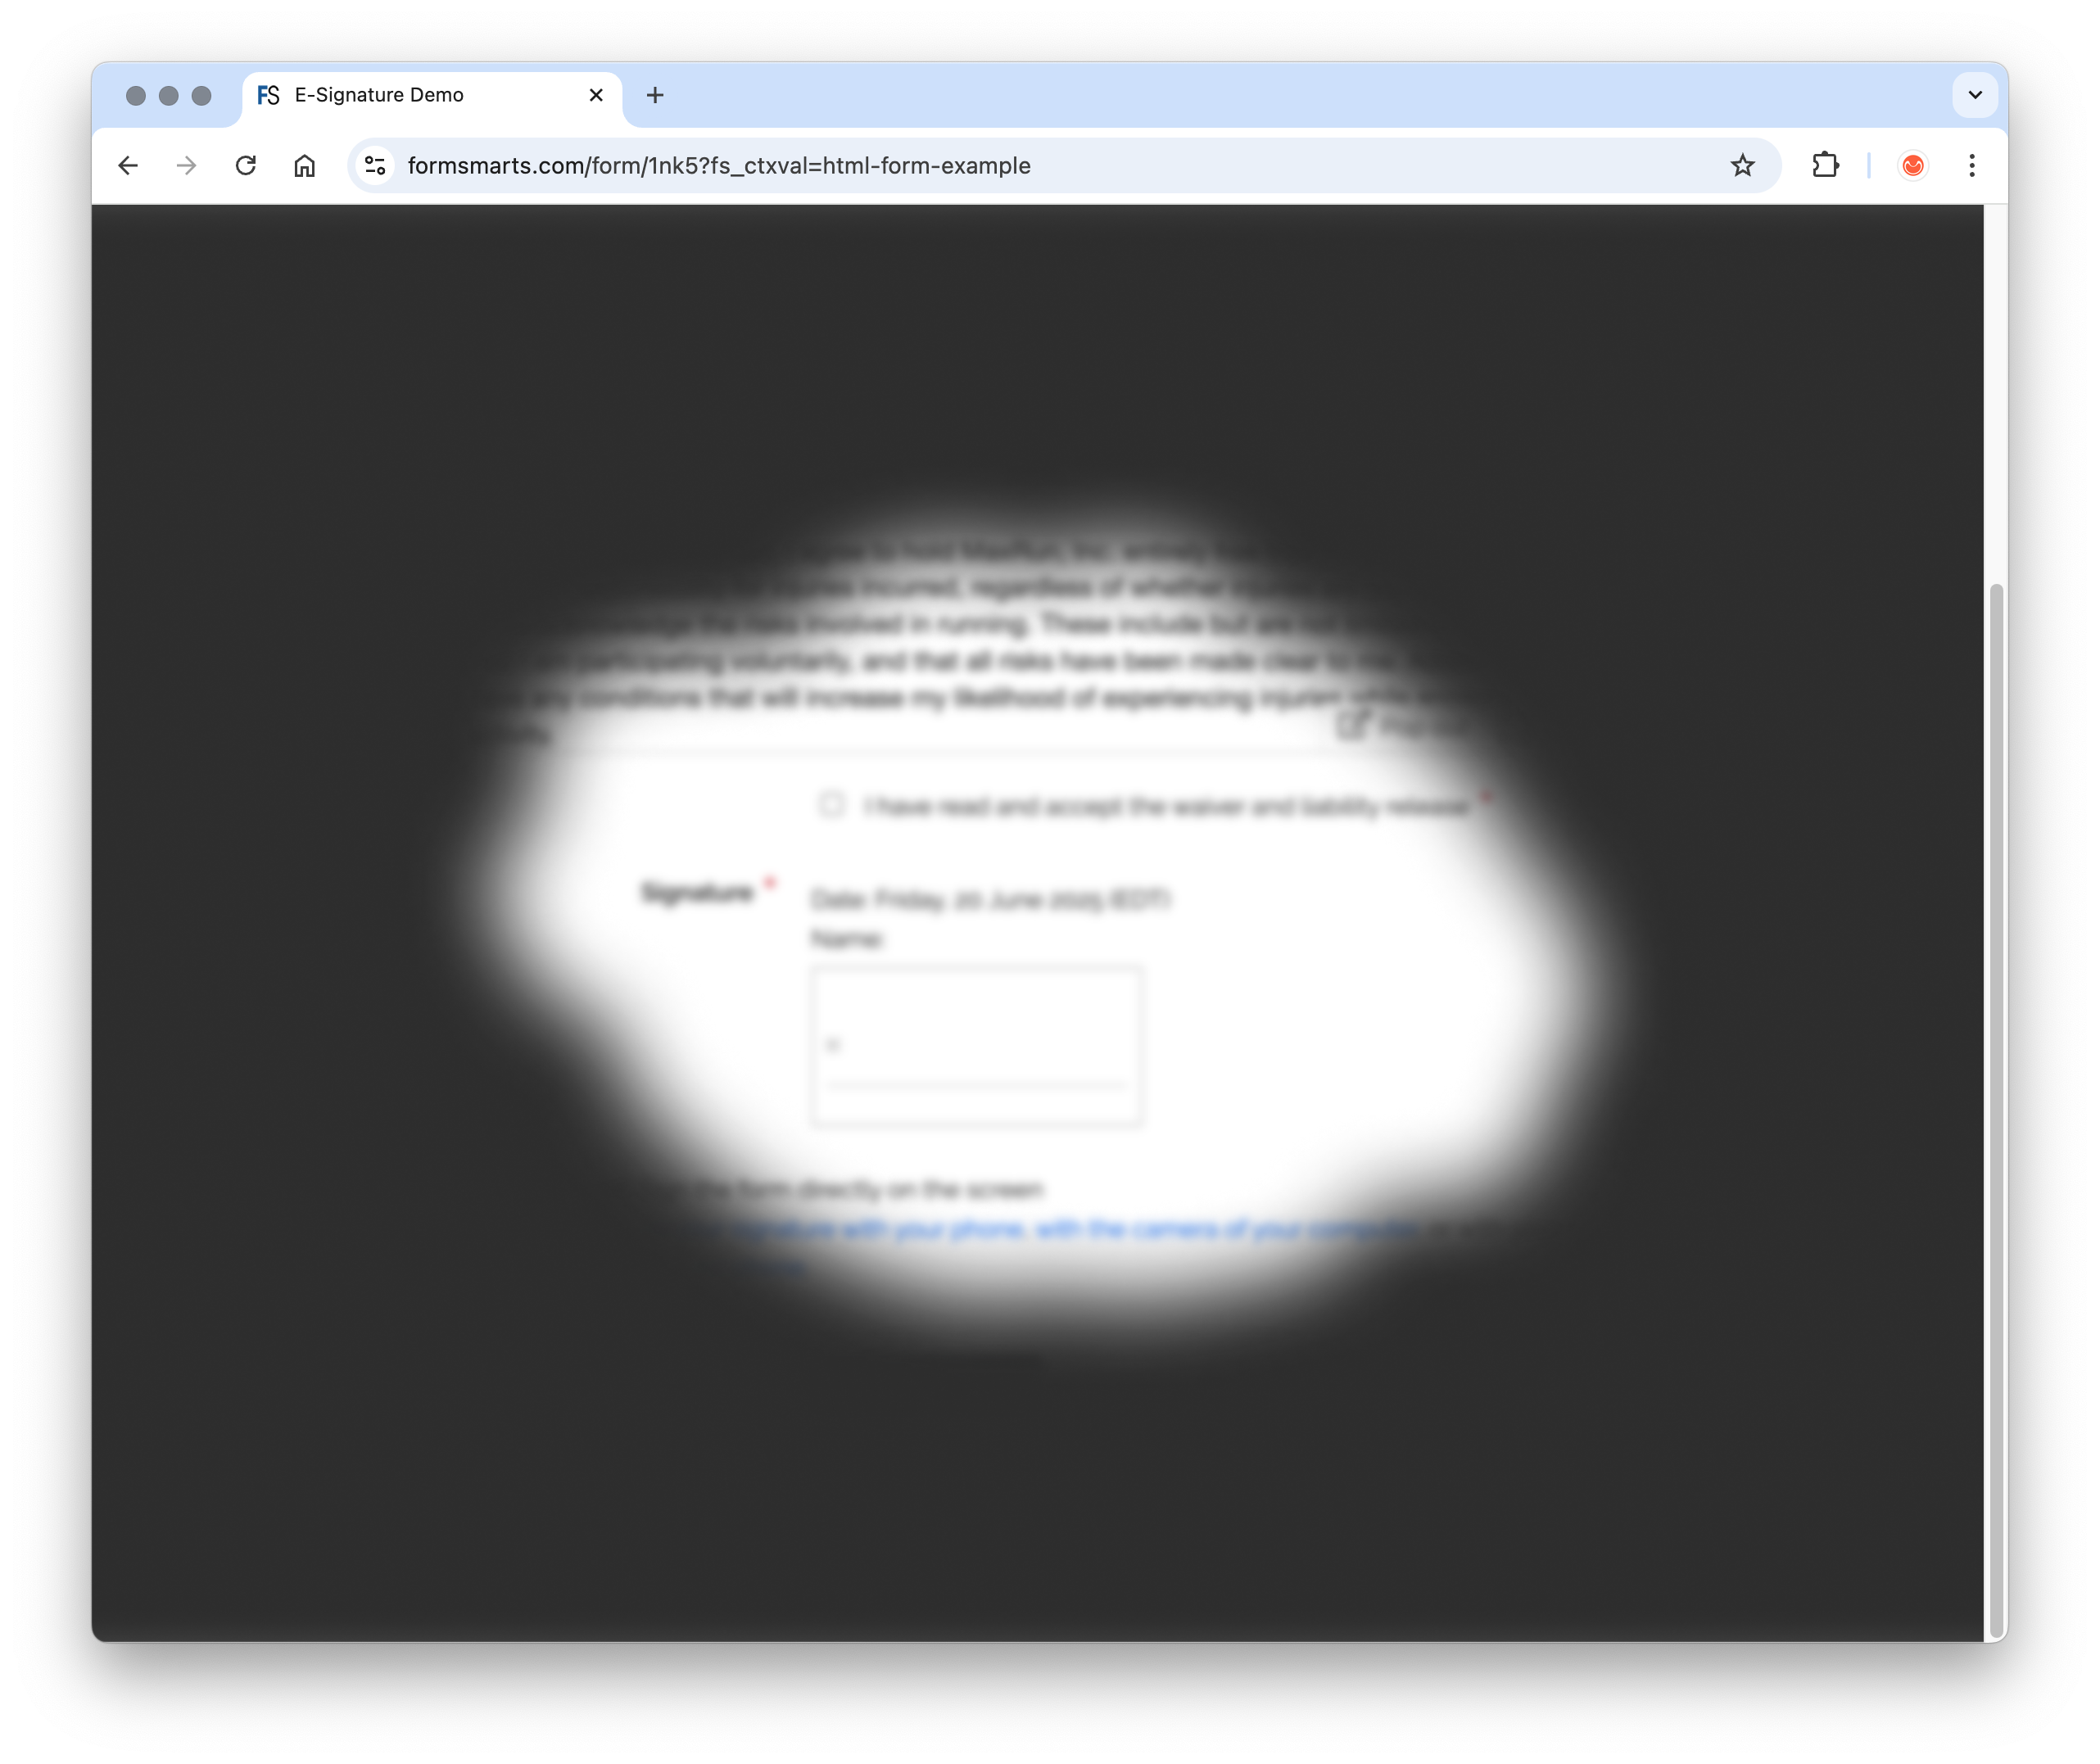
\includegraphics[width=115pt]{imgs/glaucoma-filter.png}
    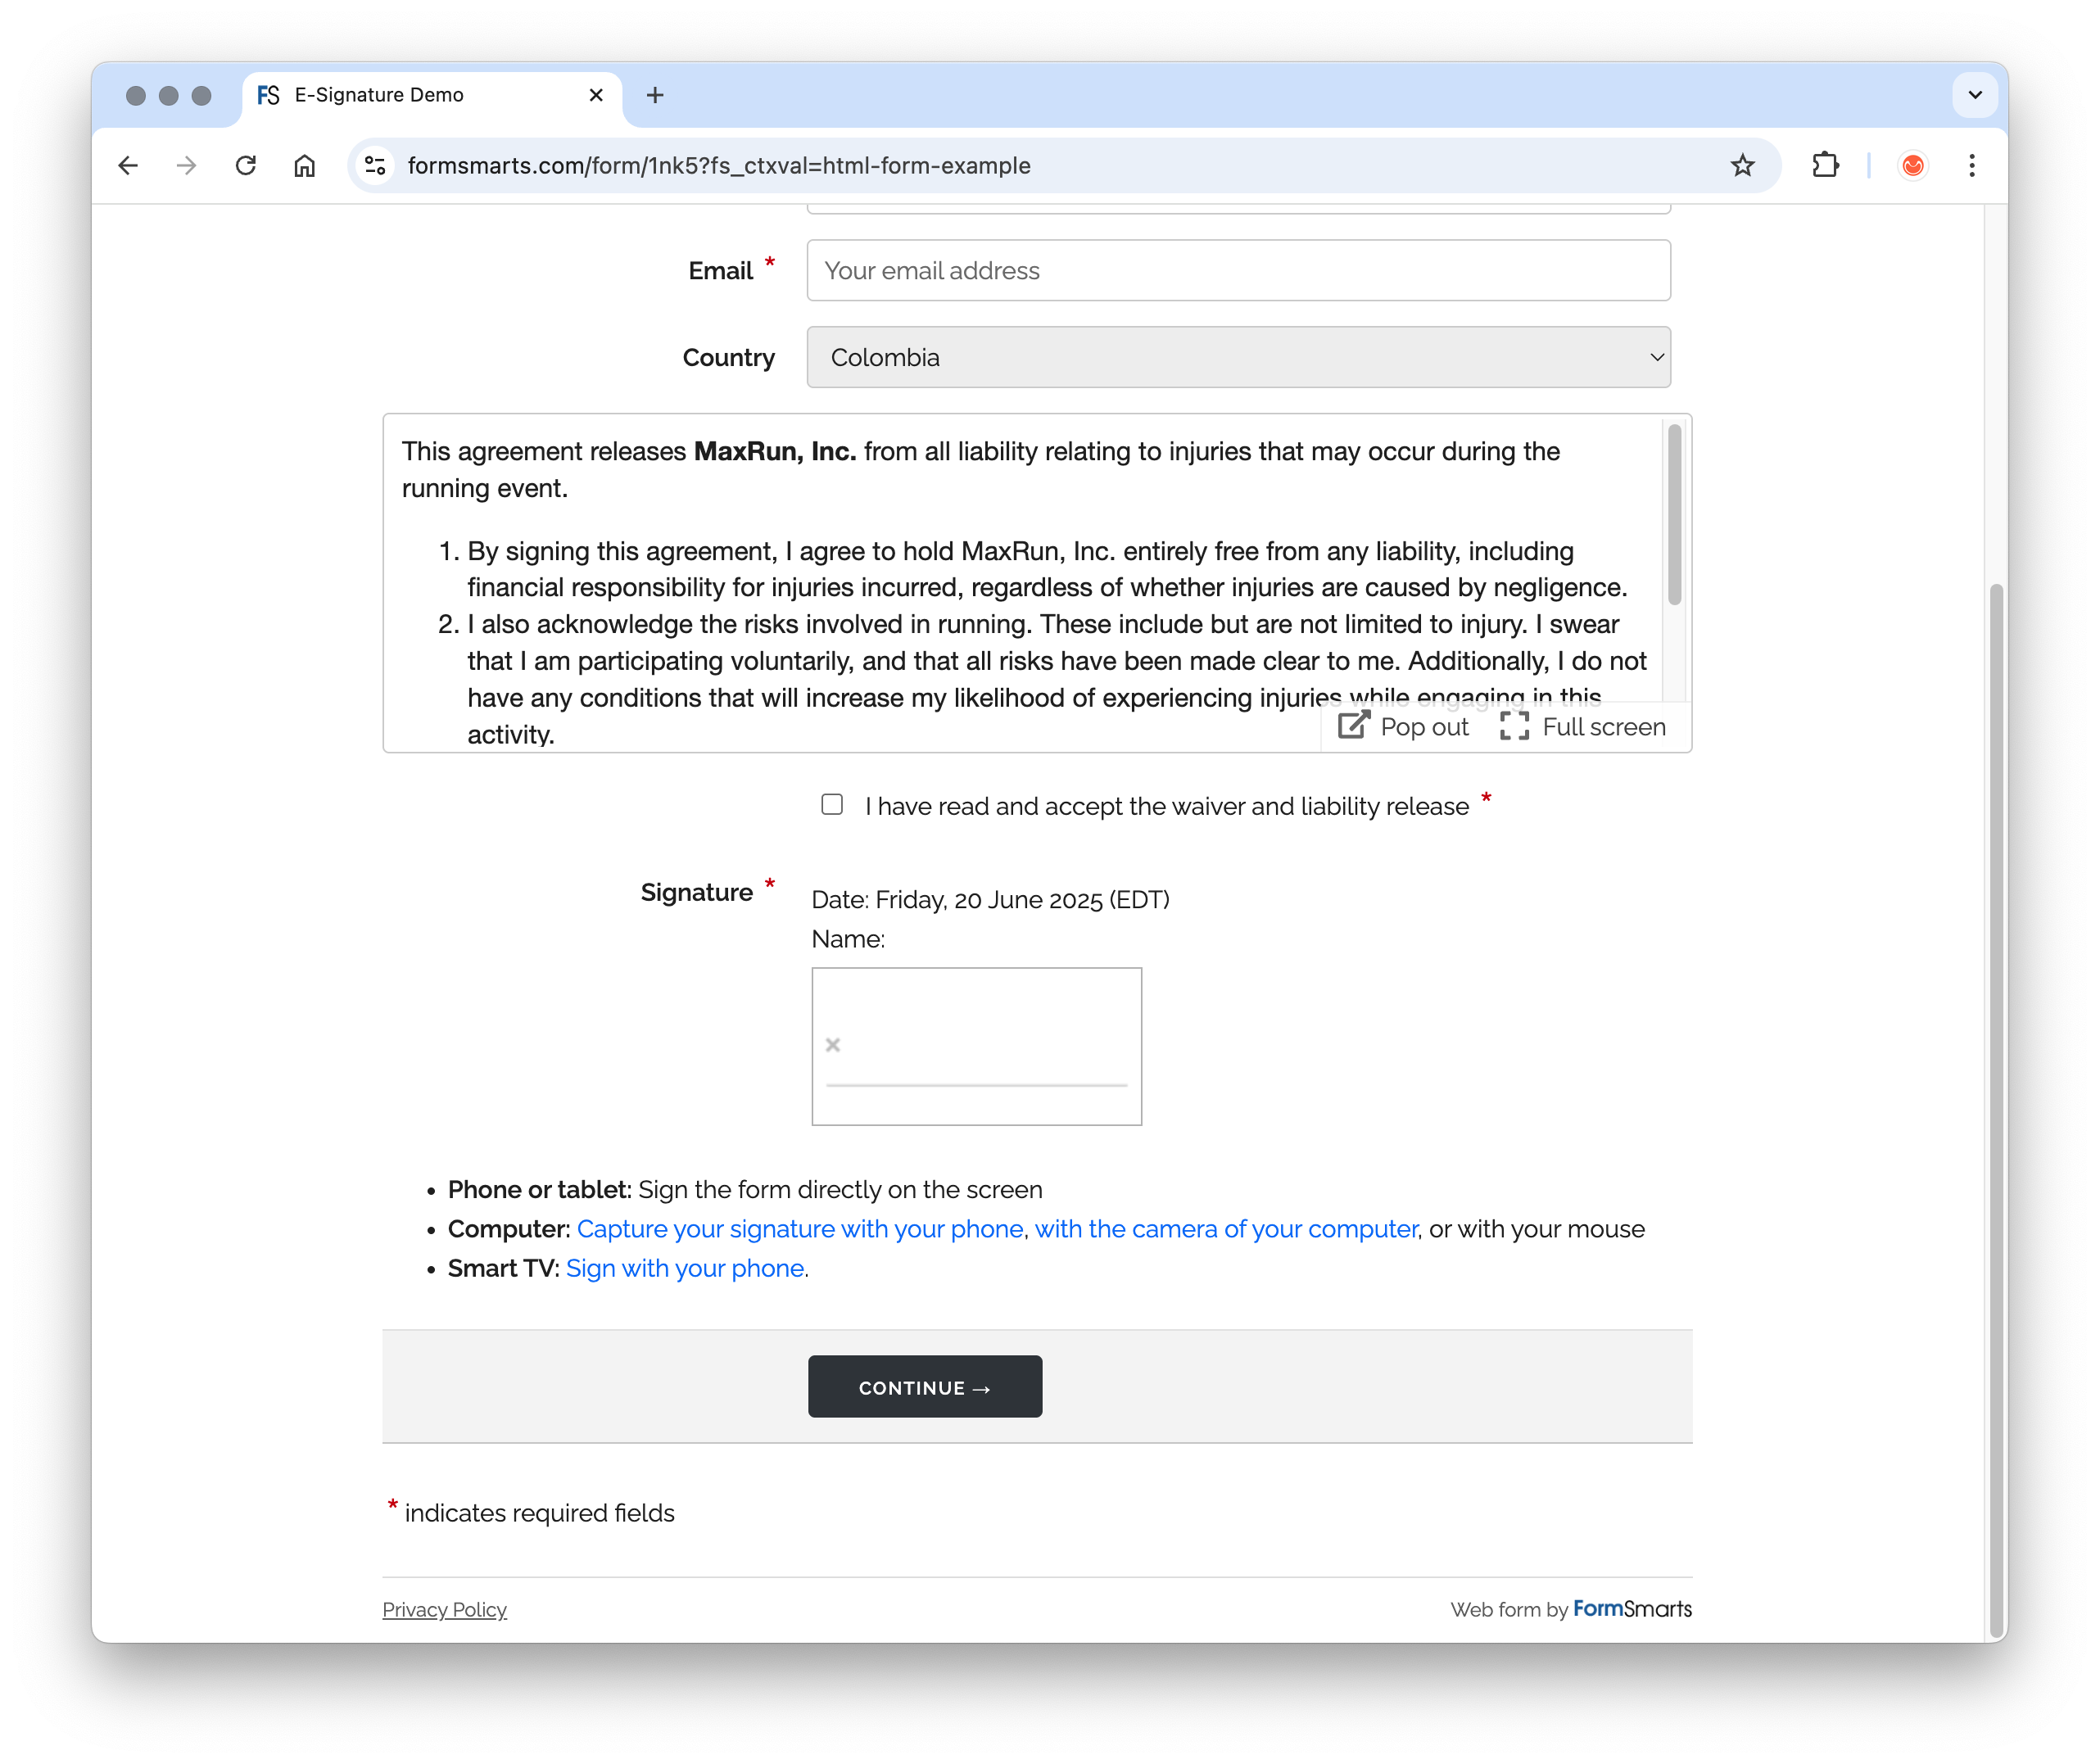
\includegraphics[width=115pt]{imgs/no-glaucoma-filter.png}
    \caption{Left: Glaucoma filter applied to an example form requiring a signature. The "Submit" button is no longer visible, making it difficult to locate. Right: Original version.}
    \vspace{-13pt}
    \label{fig:glaucoma-filters}
\end{figure}

\begin{figure}
    \centering
    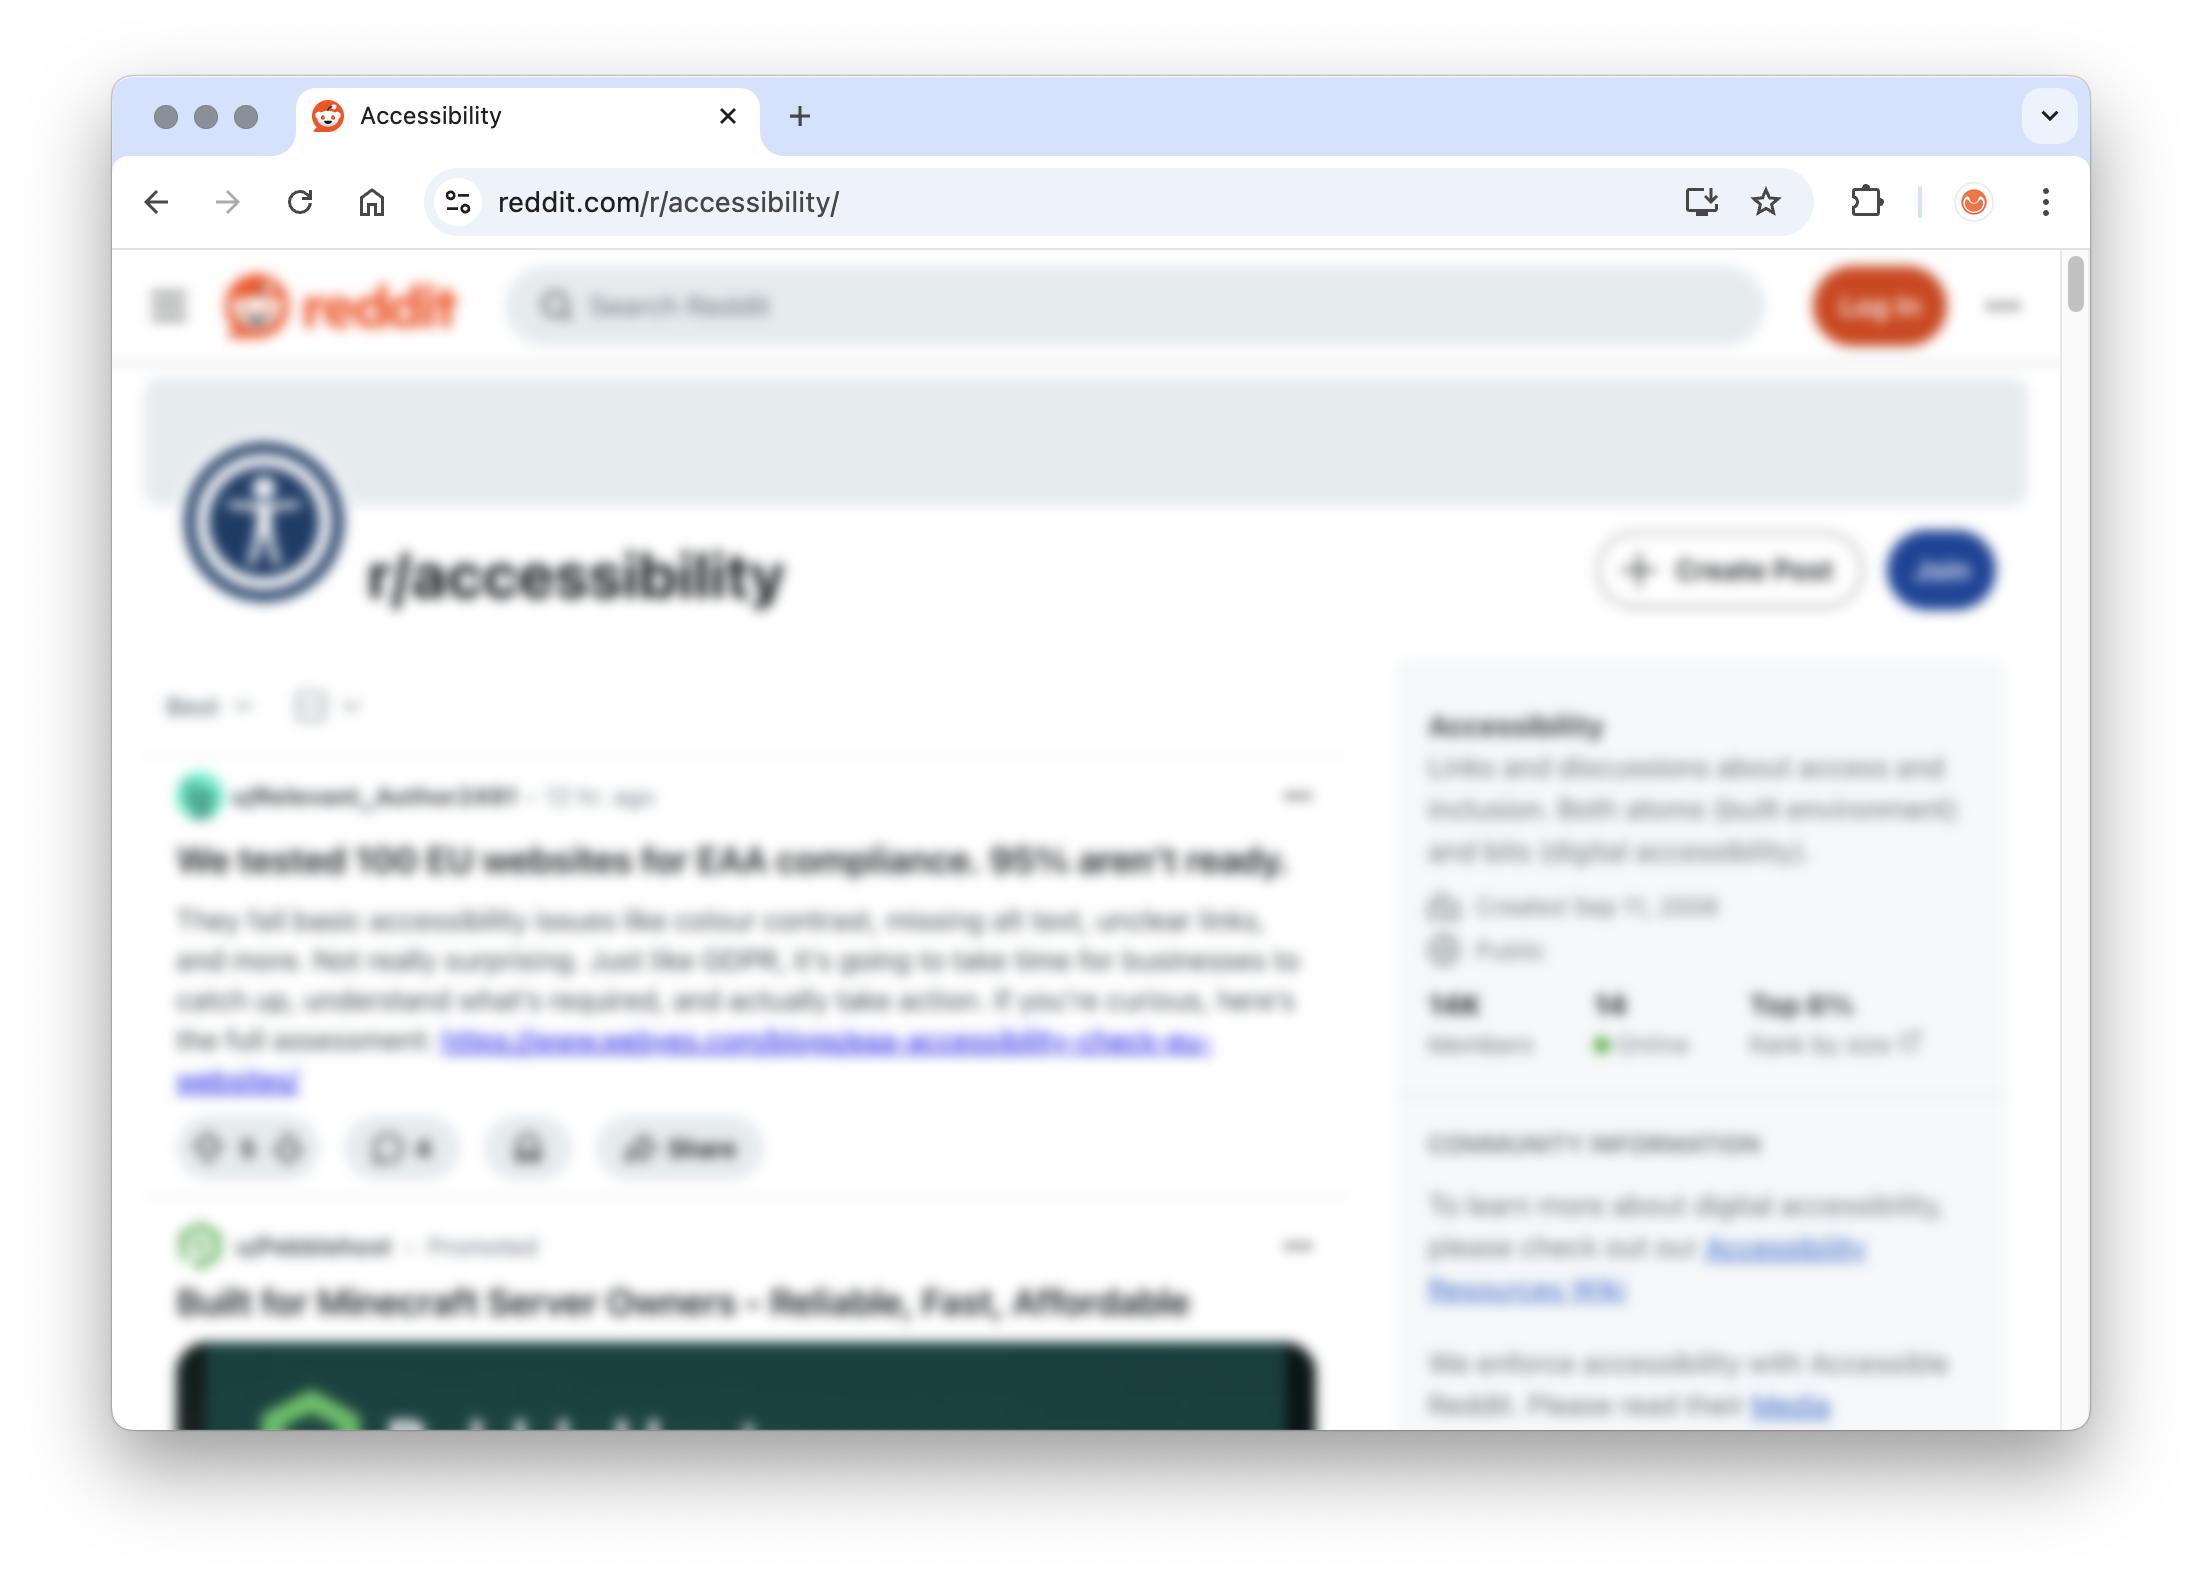
\includegraphics[width=115pt]{imgs/myopia-filter.png}
    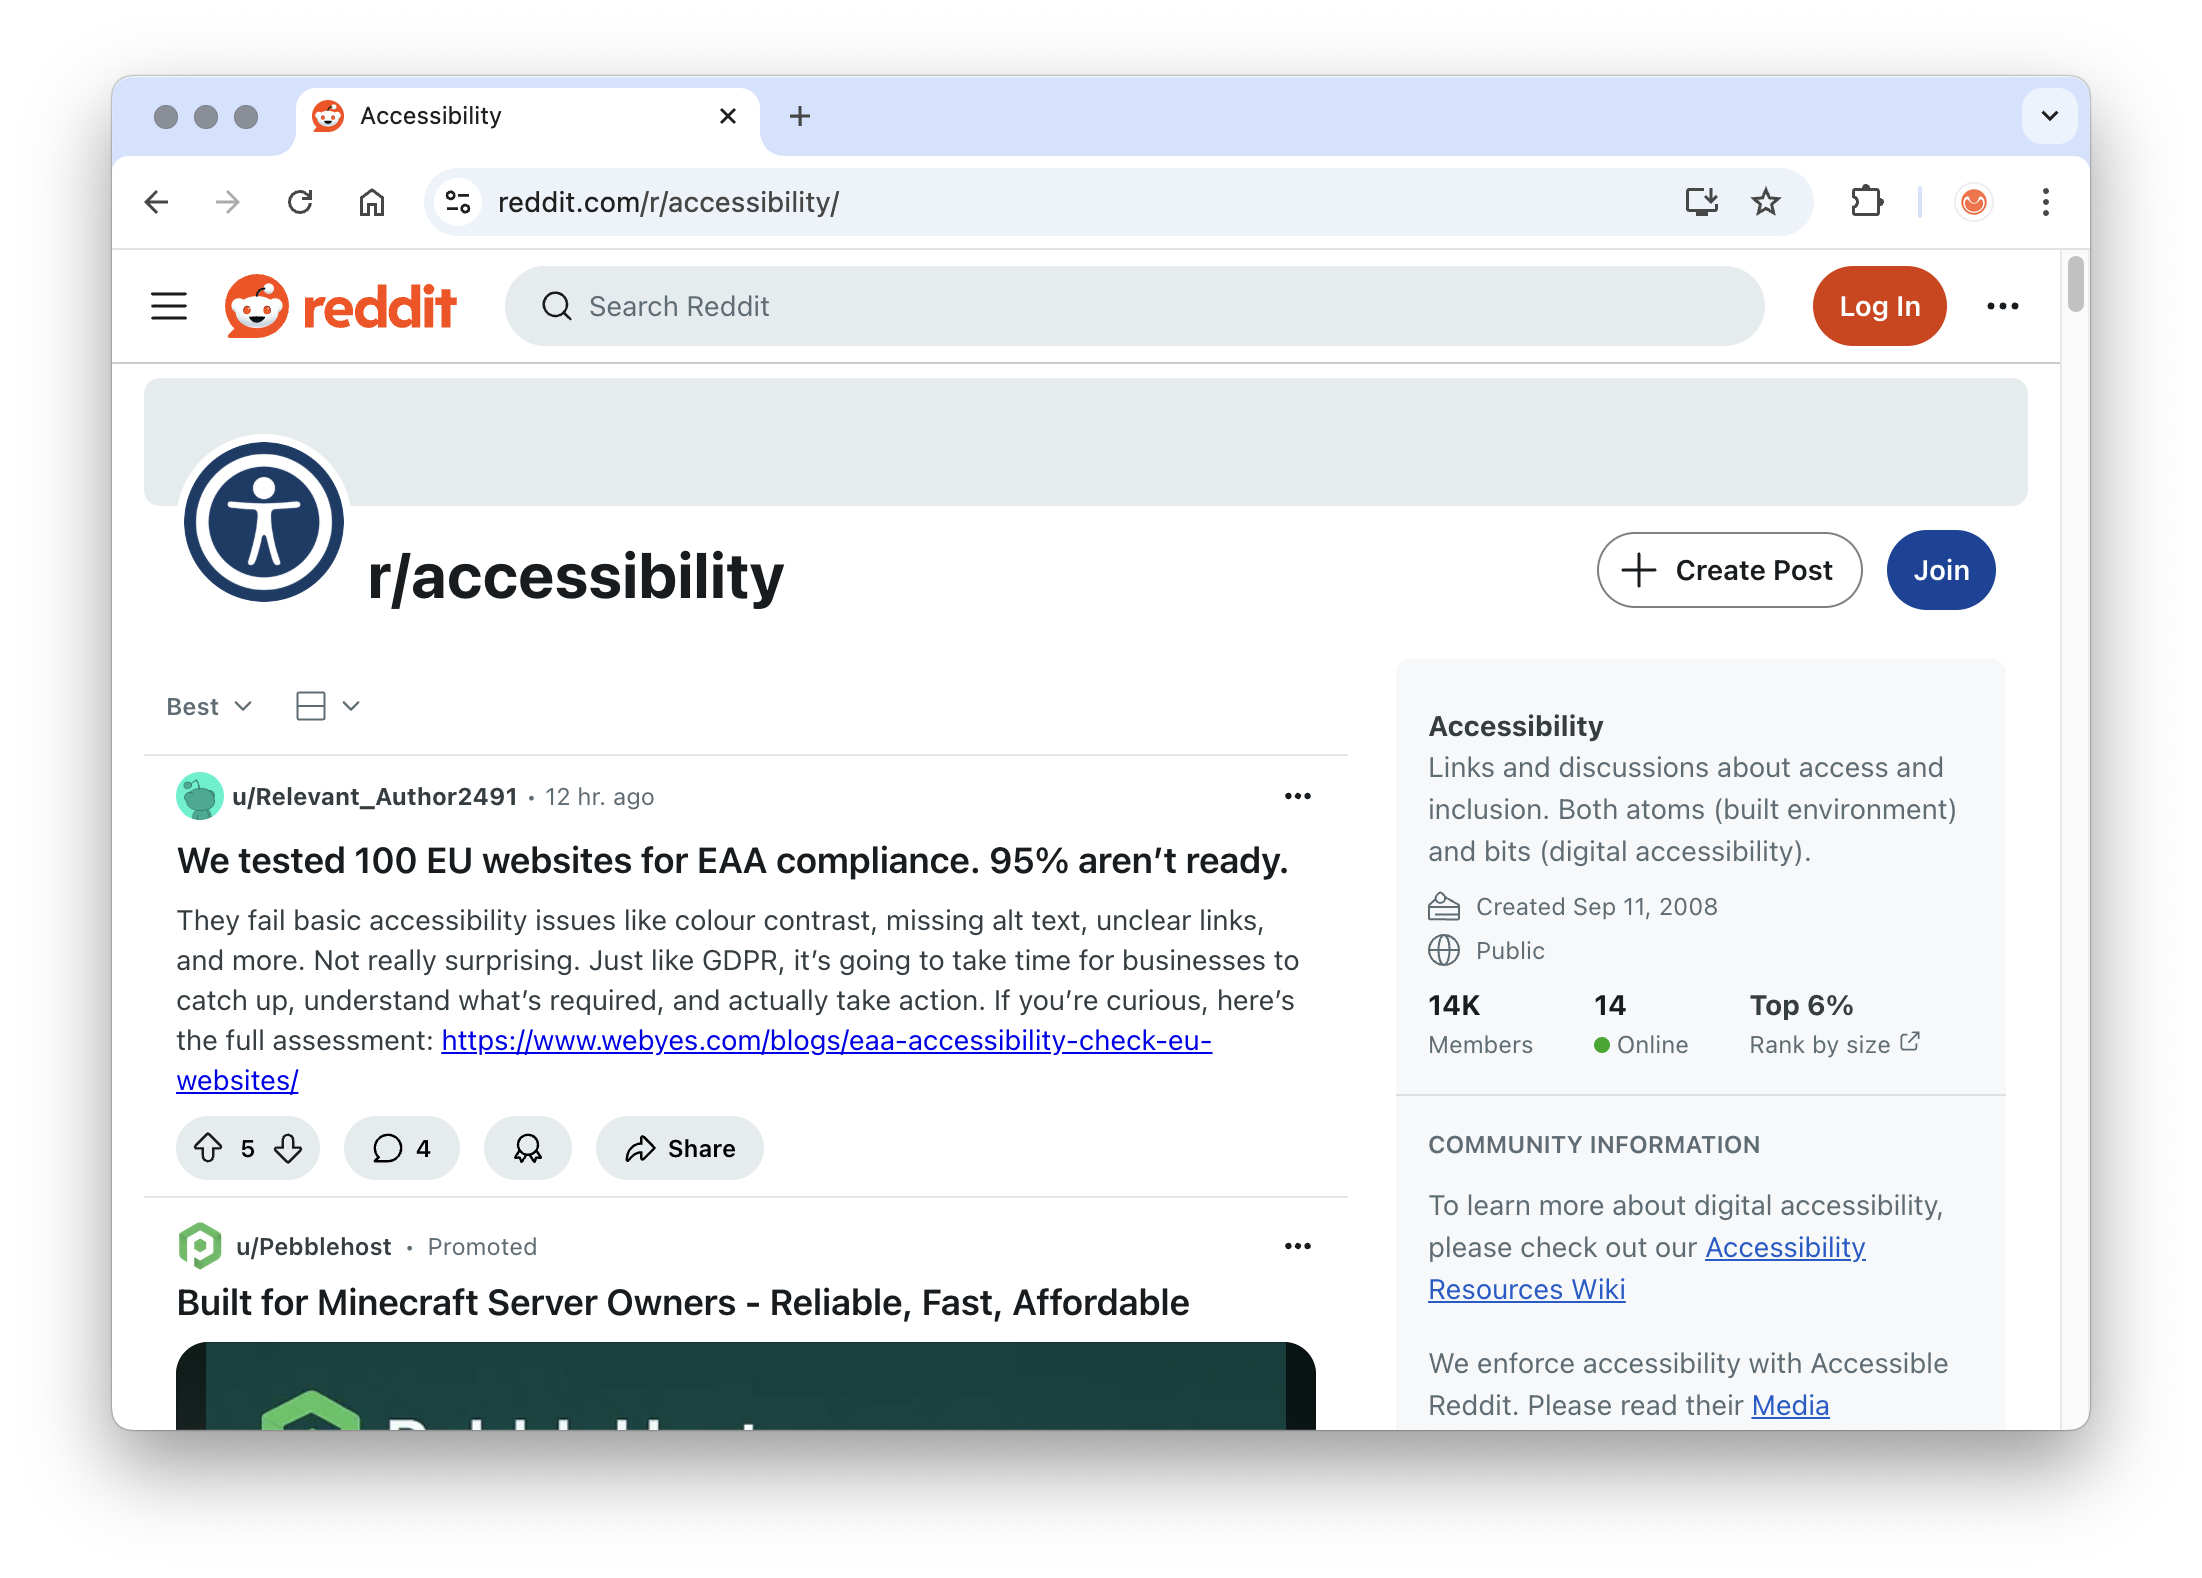
\includegraphics[width=115pt]{imgs/no-myopia-filter.png}
    \caption{Left: Myopia filter (-3 diopters) applied to a social media webpage, reducing clarity and edge sharpness. Right: Original version.}
    \vspace{-13pt}
    \label{fig:myopia-filters}
\end{figure}

These simulations (see figures. \ref{fig:glaucoma-filters} and \ref{fig:myopia-filters}) were implemented using the Visual Impairments Simulator Chrome extension \cite{visual_impairments_simulator}. While such tools provide a useful approximation of typical visual conditions, they are inherently limited: visual disabilities are highly individualized, and no filter can perfectly replicate the subjective visual experience of every user.

In addition, experimenting with different viewports, font sizes, and other browser configurations\cite{chiou2024automatically} will be done to test how these factors affect usability.

Future work should involve collaboration with ophthalmologists and vision science experts to improve the clinical accuracy of these filters. Their insight can guide the calibration of filter parameters and help us design simulations that more closely resemble the lived experiences of users.

\subsection{Assistive output integration}

\begin{figure}
    \centering
    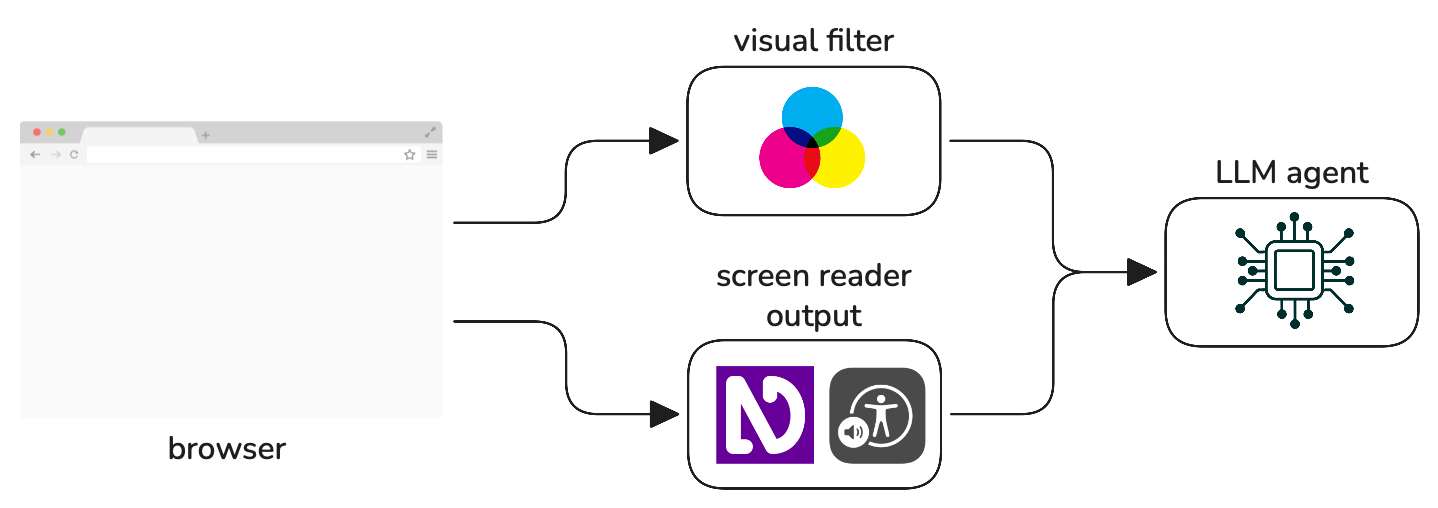
\includegraphics[width=1\linewidth]{imgs/flow.png}
    \caption{Proposed pipeline for the agent feeding inputs}
    \vspace{-13pt}
\label{fig:pipeline}
\end{figure}


The agent must capture what an assistive technology user would hear and do. For screen reader output, we can integrate a driver API, such as Guidepup\cite{guidepup2025} that programmatically controls VoiceOver (macOS)\cite{voiceover2024} or NVDA (Windows)\cite{nvda2024}.
This driver issues the same keyboard commands a user would and exposes the spoken utterances\cite{guidepup2025}. The agent framework would invoke this API at each step and record the resulting string of text (including element role, name, state) as sensory input.

For keyboard-only navigation logs, the agent can log focus events. As the agent presses Tab, arrow keys, Enter, etc., a browser automation framework, such as Playwright\cite{playwright2025}, Selenium\cite{garcia2024selenium}, or Kraken\cite{ravelo2023kraken}, can attach listeners to record each focus transition and action. This yields a sequence of elements visited in order\cite{ravelo2023kraken}. 
These logs serve two purposes: they ensure the agent only uses keyboard input, and they provide a trace of the navigation path for later analysis and execution. For instance, the log can reveal if an item was skipped or if the focus order was non-standard. Together, these multimodal streams visual focus shifts and spoken labels populate the agent's perception at each timestep. 

The agent may optionally inspect the page for \ac{a11y} metadata, thereby having the ability to cross-check perception. This means reading the ARIA attributes for the current focused element. For instance, when an element is in focus, the agent can query its ARIA label, via de \ac{AOM} or other APIs. This is then compared to the other information (visual, audio). If the visible text of a button says “Search” but its ARIA label is “Submit,” that mismatch is noteworthy. Likewise, this is helpful for alt text. If the alt text of an image is "Company Logo" but the screen reader says "Image", it indicates a missing accessible name. This is useful for verifying consistency, which is one of the guidelines on \ac{WCAG} and IBM's\cite{ibm2025accessibility}. 

\subsection{Decision and Action Module}

Our approach consists of prompting the agent with a basic user goal, such as “given this screenshot and screen reader transcript, where is the 'Submit' button?” The agent will then attempt to complete the task, using the screen reader and seeing through the visual impairment filter applied to the interface.

For example, one scenario may involve an \ac{AI} agent attempting to find and click a "Submit" button after filling out a form. With a glaucoma filter applied (see Fig. \ref{fig:glaucoma-filters}), the button may become difficult to distinguish due to peripheral blur or low contrast. The agent has to decide which interaction method works best (pointer, keyboard, etc) and execute the decision.

\subsection{Workflow Definition}

Each testing task needs to be defined in advance. This can be done either with a script or using natural language to define a goal. Then, the agent will execute said task in a closed loop that has a completion or failure condition. All in all, the loop can be structured in this way (see figure \ref{fig:pipeline}).

\underline{Steps:} Perception (capture current \ac{UI} state: screenshot, screen-reader output, optionally DOM/ARIA information) $\rightarrow$ Decision (agent chooses next action, e.g., LLM generates plan and writes a rule-based script that framework follows) $\rightarrow$ Action (execute step) $\rightarrow$ Measure (log outputs, check goal, repeat if needed).


\subsection{Metrics and Analysis}

After execution is complete, some of the metrics we propose that the system displays are both classic usability and accessibility-specific. These include the agent's task success rate, efficiency (measured by completion time or number of actions), and the frequency of interaction errors such as missed clicks or incorrect actions that require backtracking. 

We also include the consistency between screen reader output and the visible \ac{UI}, flagging any mismatches between spoken labels and on-screen text or roles. Visual robustness can also be examined by analyzing the webpage before the filter, discovering layout faults like overlapping or off-screen elements, among others. 

Heuristic checks are performed during testing, such as verifying that text scales appropriately in high-contrast or large-text modes and monitoring for navigation loops. Throughout the process, we aggregate logs of the agent's actions and screen reader output for offline analysis, enabling manual review or further explanation by the agent. By comparing these metrics across different simulated conditions, we can quantify the impact of visual impairments on usability and identify both layout and semantic \ac{a11y} issues.

\section{Evaluation}

To investigate the feasibility and effectiveness of using autonomous AI agents for \ac{a11y} evaluation, we pose several research questions. First, we ask whether autonomous AI agents can realistically emulate the interaction patterns of users with vision-related impairments when navigating web interfaces. This includes examining which visual filters or perceptual constraints most effectively represent different types of visual impairments in a simulated context, and what design principles are necessary for agents to approximate impaired visual perception through perception-based (rather than code-aware) interaction.

We also explore whether these agents can surface \ac{a11y} problems that static tools overlook, such as poor contrast visibility, confusing focus order, or dynamic content that is not screen-reader friendly. Another important question is whether agent-based testing, when combined with simulated impairments, can produce \ac{a11y} assessments that are reliable and generalizable. We are interested in the extent to which LLM-powered agents or learning-based systems can internalize \ac{a11y} heuristics through observation of human interaction data, rather than relying solely on static rule sets.

Finally, we investigate how combining simulated visual impairment filters with screen reader output affects the agent's ability to detect \ac{a11y} issues, and whether multi-modal input can uncover problems, such as missing alt text, that would not surface if using only visual filtering.

To evaluate our approach, we will conduct experiments on a curated set of benchmark web pages, including public sites with documented \ac{a11y} issues. Inspired by Alameer et al.\cite{alameer2016detecting}, who compiled websites with internationalization challenges, we may extend our benchmarks to include similar cases. For each page, we will define representative tasks—such as form submission and navigation—and assess agent performance across different visual filters and input modalities. In future work, we plan to complement these quantitative results with qualitative feedback from \ac{a11y} experts and targeted user studies, to further validate the effectiveness and generalizability of agent-based \ac{a11y} testing.
